\documentclass[11pt]{article}

\usepackage[utf8]{inputenc}
\usepackage{wrapfig}
\usepackage[pdftex]{graphicx}

\newcommand{\whitespace}{\rule{\linewidth}{0.0mm}}

\begin{document}
\title{Virtual Reality}
\author{Maximilian Sieß}

%======TITLE PAGE=========
\begin{titlepage}
	\begin{center}
		
\includegraphics[scale=1]{images/uibk} \\
		Leopold-Franzens-Universität Innsbruck
		\linebreak 

		Institute of Computer Science \\
		Interactive Graphics and Simulation Group
		%\maketitle
	
		\whitespace \\[2.0cm]
		\LARGE \textbf{Virtual Reality}\\
		\normalsize Einführung in das Wissenschaftliche Arbeiten\\
		Seminarreport
	
		\whitespace \\[0.8cm]
		Maximilian Sieß
		
		\whitespace \\[2.0cm]
		advised by\\
		Prof. Dr. Matthias Harders
		
		\whitespace \\[4.0cm]
		Innsbruck, \today

	\end{center}
\end{titlepage}

%\newpage 

%=========TABLE OF CONTENTS==============
%\tableofcontents


\newpage
\section{Abstract}
The dream of feeling present at another location than one actually is at is becoming reality with the advent of virtual reality developments. Display technology, software and input devices have evolved enough to make this dream possible enough to be exciting and useful in many different areas. The drawbacks to them that still prevent the user to fully forget that they are seeing a simulation realized by computer graphics get diminished more and more, increasing the intensity of the intended effect.


\section{Introduction}
Virtual Reality is the attempt to use technology, such as head mounted display devices, and computer generated graphics, to allow the user to experience a sense of presence in a virtual environment.  This is used in a wide variety of cases, including but not limited to entertainment, education, medical therapy, research, and visualization. Virtual Reality has the potential to fundamentally change the way we experience, and interact with, data and software.

	\subsection{Definitions}
		\subsubsection{Virtual Reality}
			Virtual Reality, or VR for short, is the field of computing that aims to create a virtual world, allowing the user to enter, experience and interact with it, by using specific devices to simulate the virtual environment and the feedback it would provide in order to make the experience as real as possible.
			%"Virtual Reality stands for the field of computing which has the objective of creating a virtual world, having one immerse into it and giving one the capability of interacting with this world, while using specific devices to simulate an environment and stimulate one by feedback in order to make the experience as real as possible." 
			\cite{boas13}
			
		\subsubsection{Immersion}
			Immersion can be differentiated into three different forms. \textit{Engagement}, which has to come from the subject, not the medium. \textit{Engrossment}, which depends on how the software is designed, and is important to affect a subjects emotions, if that is intended. And lastly \textit{total immersion}, or the sense of presence. Total immersion can be understood as what happens when someone is fully engulfed by a piece of media, like a book, movie, or computer game. \cite{Brown:2004:GIG:985921.986048} \\
			Total immersion can also, in the case of VR, be taken more literally as the “extent to which a person's cognitive and perceptual systems are tricked into believing they are somewhere other than their physical location”. \cite{Patrick:2000:ULP:332040.332479} Users of the Oculus Rift have been recorded to be so immersed in the simulation, that they tried to interact with virtual objects by reaching out them them, to for example touch or grab them. \cite{bastiaens14}

		\subsubsection{Telepresence}
			Telepresence is defined as to have the experience that one is present at another location than his or her physical one.  This name has been coined by Marvin Minsky in the 1980s. \cite{minsky1980telepresence} While Minsky's definition had in mind that ones actions have consequences at another physical location somewhere, which is not necessarily true for VR, Virtual Reality follows the same concept.
			
\section{Related Work}
	\subsection{Technology}
	\subsubsection{Head-Mounted Displays}
	
	\begin{wrapfigure}{r}{0.5\textwidth}
		\vspace{-20pt}
		\begin{center}
			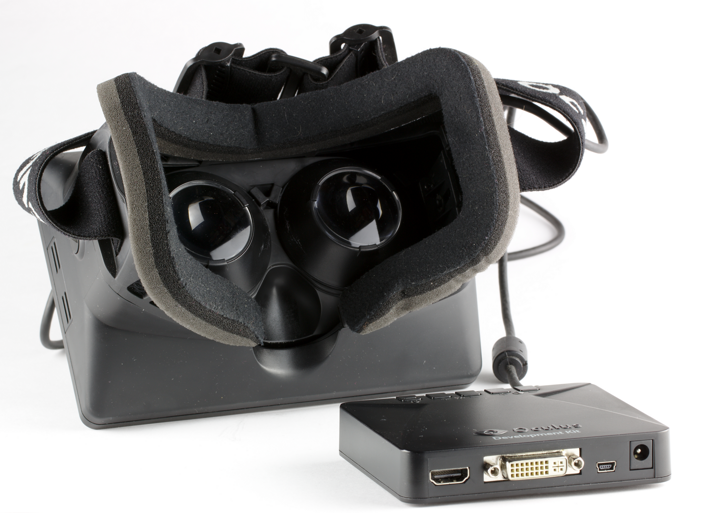
\includegraphics[scale=0.3]{images/or_small.png}
		\end{center}			
		\vspace{-20pt}
			\caption{A Oculus Rift DK1 Headset and HDMI/DVI Converter Box}
		\vspace{-10pt}
	\end{wrapfigure}
	
		Today, the most common form of how Virtual Reality is realized is via head-mounted displays. Goggles with a high density display in it, the same as used in phones. Utilizing special lenses and stereoscopic vision to create a believable view into the virtual environment. \\
		Examples for headsets like these would be the \emph{Oculus Rift} by Oculus VR and one under the working title of \emph{Project Morpheus} by Sony. Both are very similar in execution and produce a VR experience of similar quality. \cite{goradia2014review}
	
	
	At the time of this writing, both have not seen a commercial release, although a development kit for the Oculus Rift is available for purchase.

	\subsubsection{Software}
		Programming software for virtual reality does not differ much from regular computer graphics programming. Most commercial vendors offer their own API that helps translating a virtual camera to a two camera 3D setup. It was found however, that how the camera is used is imperative to not give the user of the virtual reality headset motion sickness or other unpleasant side effects. \cite{seppanen14}
		
		
		For example, moving the camera without the user moving their head has resulted in severely negative feedback from users. The Oculus Rift Best Practices Manual states that "Acceleration creates a mismatch among your visual, vestibular, and proprioceptive senses; minimize the duration and frequency of such conflicts. Make accelerations as short (preferably instantaneous) and infrequent as you can." \cite{yao2014oculus}
	
	\subsubsection{Input Devices}
	With headmounted displays, vision, the groundwork for a feeling of presence in virtual reality, is laid out. Headsets or surround sound systems have been shown to suffice for the audio representation of the virtual environment.\\
	Moving around naturally has proven difficult, however. While virtual reality demos often use a gamepad, it is less than ideal for upholding a sense of presence. The abstract translation from a analogue stick to moving oneself in virtual space, or interact with one's surroundings, is not very intuitive. \cite{ruddle13} Some of the earliest virtual reality input devices were wired gloves, using fiber optics, conductive ink and mechanical sensors to determine the state of the users hands. \cite{boas13} Other, later developments were done with wands, like the Nintendo Wii motion-sensor controller or the Sony Move Controller. \cite{boas13} And another way to realise input is to use computer vision, by using 3D cameras that record infrared, or end user devices such as the Microsoft Kinect, or the Sony Playstation Eye. \cite{boas13}
	
	\subsection{Applications of Virtual Reality}
	Most virtual reality hardware developed at this time is geared towards the entertainment business, with a special focus on simulation software, such as flight simulators, and video games. %From Oculus Rift, over Sony's Project Morpheus to Vive by HTC and Valve.
	Yet VR can also be used for more humanitarian ways or scientific studies. Games made for these purposes are called \emph{serious games}, and are being used to, for example, allow the user to examine scanned, centuries old manuscripts of which only one copy exists, at a virtual table. \cite{lorenzini2013serious}
	
	Virtual reality can be used to visualize and teach subjects in ways that were inaccessible before. Teaching history by visiting locations or events of historical importance, for example. \cite{mosaker2001visualising}
	
	Interest in virtual reality for training simulation purposes by the military is one of the most important one when it comes to investment and deployment. \cite{moshell1993three}
	
	Perhaps unexpected are the numerous ways virtual reality was found to be useful in medical treatments. From distracting patients from intense pain during treatments, by allowing them to feel like they are somewhere else \cite{hoffman14}, %over teaching walk-inhibited patients to walk again \cite{ruddle13}, 
	to help patients with Diplopia (commenly known as lazy eye) to see three dimensionally again and potentially even improve their vision. \cite{blaha2014diplopia}

\section{Discussion}
With head-mounted displays, headphones and gloves, suspension of disbelief is easier than it ever has been before. All these technologies seem to work towards the same goal, to have total immersion without any barriers diminishing the feeling of presence.

At the moment, there are still many of these barriers remaining. The lack of intuitive input devices, the small imperfections of current head-mounted displays, and not very far research of virtual reality software. However, total immersion is being reported by users to be reached at least most of the time. \cite{bastiaens14}

\section{Conclusion}
The level of immersion achievable by technology available today, namely the Oculus Rift Development Kit, is already enough to use virtual reality effectively already, as many studies and experiments have shown.

Once the first VR headset is commercially released for end users, even more applications and developments are going to find new and innovative ways to use telepresence and total immersion in beneficial, innovative, or simply entertaining ways.


\bibliographystyle{plain}
\bibliography{vr_bib}

\end{document}

%Todo still:
%insert more pictury pictures
%polish!
%done.


